\documentclass[bachelor, och, diploma]{SCWorks}
% параметр - тип обучения - одно из значений:
%    spec     - специальность
%    bachelor - бакалавриат (по умолчанию)
%    master   - магистратура
% параметр - форма обучения - одно из значений:
%    och   - очное (по умолчанию)
%    zaoch - заочное
% параметр - тип работы - одно из значений:
%    referat    - реферат
%    coursework - курсовая работа (по умолчанию)
%    diploma    - дипломная работа
%    pract      - отчет по практике
%    pract      - отчет о научно-исследовательской работе
%    autoref    - автореферат выпускной работы
%    assignment - задание на выпускную квалификационную работу
%    review     - отзыв руководителя
%    critique   - рецензия на выпускную работу
% параметр - включение шрифта
%    times    - включение шрифта Times New Roman (если установлен)
%               по умолчанию выключен
\usepackage[T2A]{fontenc}
\usepackage[cp1251]{inputenc}
\usepackage{graphicx}

\usepackage[sort,compress]{cite}
\usepackage{amsmath}
\usepackage{amssymb}
\usepackage{amsthm}
\usepackage{fancyvrb}
\usepackage{longtable}
\usepackage{array}
\usepackage[english,russian]{babel}
\usepackage{tempora}
\usepackage{minted}

\usepackage[colorlinks=true]{hyperref}


\newcommand{\eqdef}{\stackrel {\rm def}{=}}

\newtheorem{lem}{Лемма}

\begin{document}

% Кафедра (в родительном падеже)
\chair{математической кибернетики и компьютерных наук}

% Тема работы
\title{Нейронные сети}

% Курс
\course{4}

% Группа
\group{451}

% Факультет (в родительном падеже) (по умолчанию "факультета КНиИТ")
%\department{факультета КНиИТ}

% Специальность/направление код - наименование
% \napravlenie{02.03.02 "--- Фундаментальная информатика и информационные технологии}
%\napravlenie{02.03.01 "--- Математическое обеспечение и администрирование информационных систем}
%\napravlenie{09.03.01 "--- Информатика и вычислительная техника}
\napravlenie{09.03.04 "--- Программная инженерия}
%\napravlenie{10.05.01 "--- Компьютерная безопасность}

% Для студентки. Для работы студента следующая команда не нужна.
%\studenttitle{Студентки}

% Фамилия, имя, отчество в родительном падеже
\author{Озерова Данилы Николаевича}

% Заведующий кафедрой
\chtitle{к.\,ф.-м.\,н.} % степень, звание
\chname{С.\,В.\,Миронов}

%Научный руководитель (для реферата преподаватель проверяющий работу)
\satitle{доцент, к.\,ф.-м.\,н.} %должность, степень, звание
\saname{С.\,В.\,Миронов}

% Руководитель практики от организации (только для практики,
% для остальных типов работ не используется)
\patitle{к.\,ф.-м.\,н., доцент}
\paname{Д.\,Ю.\,Петров}

% Семестр (только для практики, для остальных
% типов работ не используется)
\term{2}

% Наименование практики (только для практики, для остальных
% типов работ не используется)
\practtype{учебная}

% Продолжительность практики (количество недель) (только для практики,
% для остальных типов работ не используется)
\duration{2}

% Даты начала и окончания практики (только для практики, для остальных
% типов работ не используется)
\practStart{01.07.2016}
\practFinish{14.07.2016}

% Год выполнения отчета
\date{2023}

\maketitle

% Включение нумерации рисунков, формул и таблиц по разделам
% (по умолчанию - нумерация сквозная)
% (допускается оба вида нумерации)
%\secNumbering


\tableofcontents

% Раздел "Обозначения и сокращения". Может отсутствовать в работе
\abbreviations
% \begin{description}
%     \item $|A|$  "--- количество элементов в конечном множестве $A$;
%     \item $\det B$  "--- определитель матрицы $B$;
%     \item ИНС "--- Искусственная нейронная сеть;
%     \item FANN "--- Feedforward Artifitial Neural Network
% \end{description}

% Раздел "Определения". Может отсутствовать в работе
%\definitions

% Раздел "Определения, обозначения и сокращения". Может отсутствовать в работе.
% Если присутствует, то заменяет собой разделы "Обозначения и сокращения" и "Определения"
%\defabbr


% Раздел "Введение"
\intro
В современном мире практически на все, что мы покупаем или потребляем в той или иной форме влияют рекомендации, будь то от друзей, рекламы или, как стало с недавнего времени, от источников предложения товаров. Например, платформа Кинопоиск или Озон предлагают список фильмов и товаров, которые по мнению сервиса могут приглянутся пользователю. 
Большинство ранних рекомендательных моделей пыталась разделить пользователей на стереотипные группы, чтобы рекомендовать данной группе один и тот же товар. Примером такой работы может служить система библиотекаря Гранди []. Однако быстро такой подход получил критику в научном мире, поскольку «люди очень слабы в изучении и описании собственных когнитивных процессов» []. По исследованиям люди часто подчеркивают свои отличительные качества, что затрудняет работу по созданию стереотипов.

Таким образом можно сделать предположение, что предоставление качественных рекомендаций лежит в основе успешности работы современного бизнеса. 

Цель итоговой аттестационной работы --- изучение и построение различных моделей рекомендательных систем в области сервиса по просмотру анимации в стиле аниме, направленных на предсказание наиболее вероятных аниме, подходящих пользователю. В данной работе под моделью понимается ряд шагов, выполнение которых приведет к построению наиболее эффективной рекомендательной системы в рассматриваемой предметной области. 

Поставленная цель определила следующие задачи:
\begin{itemize}
	\item Выбрать данные для обучения и тестирования модели, провести их анализ.
	\item Построить различные модели рекомендательной системы.
	\item Протестировать качество прогнозирования.
\end{itemize}

\section{Теоретическая часть}
Основную часть данной работы составляет построение и анализ алгоритмов построения рекомендательных систем. В качестве предметной области была выбрана область стримингового сервиса аниме-фильмов.

Объектом исследования стал процесс прогнозирования интересов пользователя стримингового аниме сервиса. Предметом исследования работы является разработка модели для реализации рекомендательной системы, прогнозирующей интересы пользователя на основе просмотренных аниме.

\subsection{Коллаборативная фильтрация}
Современные подходы к построению рекомендательных систем используют либо коллаборативную (совместную) фильтрацию, либо фильтрацию на основе контента. Данные методы строят модель на основе прошлых данных о пользователе в системе, а также похожих решений, принятых другими пользователями.

В данной работе ставится цель создать рекомендательную систему для информирования пользователя об аниме, которые ему могут быть интересны. Предметом рекомендации является аниме, источник рекомендации - аудитория. Тип рекомендательной системы - коллаборативная на основе пользователей (user-based). Поскольку появление новых пользователей и аниме вынуждают выполнять перерасчет системы, то user-based тип системы более подходит данной предметной области, поскольку аниме, к примеру, добавляются в систему реже, чем пользователи.

К проблемам совместной фильтрации исследование [] относит проблему холодного старта (недостатка данных при запуске системы), однако в данном случае используется начальный большой датасет с популярного интернет-портала, поэтому данная проблема несущественна.

Совместная фильтрация успешно используется в смежных предметных областях в проектах ???, что дает возможность высказать предположение об эффективности при решении поставленной задачи.

Работа начинается с построения и анализа примитивной модели, когда для всех пар возвращаемое значение равно среднему рейтингу. Затем проводится улучшение модели на такую, которая выводит среднюю оценку между всеми пользователями, которые его оценили. В следующей модели производится следующая модификация: оценкам пользователей добавляется вес, то есть модель отдает предпочтение тем пользователям, чьи оценки похожи на рассматриваемого пользователя. Определим описанный вес так:

$$\bar r_{ua} = \frac{1}{\sum_{u', u' \neq u} s_{uu'}}  \sum_{u', u' \neq u} s_{uu'}r_{u'a}$$, где 

$\bar r_{ua}$ --- это предполагаемая оценка товара $a$ пользователем $u$, $s_{uu'}$ --- коэффициент похожести $u$ на $u'$, $r_{u'a}$ означает оценку пользователем $u'$ товара $a$.

В данной модели учитывался рейтинг каждого пользователя для прогноза окончательного рейтинга. Выдвинем гипотезу, что группировка пользователей с помощью кластеризации улучшит результат. Самая популярная реализация алгоритма основана на принципе k ближайших соседей. Она позволит выбрать k пользователей с наиболее похожими интересами относительно рассматриваемого человека. Далее данный метод предполагает выбор меры в отношении рассматриваемого пользователя и выбор k наибольших. После подсчета меры для каждого из пользователей производится умножение меры на его оценки. Затем для каждого аниме следует подсчитать сумму калиброванных оценок k наиболее близких пользователей, а затем эту сумму разделить на сумму мер k выбранных пользователей. 

$$\bar r_{ua} = \frac{1}{\sum_{u' \in N(A)} s_{uu'}}  \sum_{u' \in N(A)} s_{ai}r_{ij}$$, где 

$\bar r_{ua}$ --- это предполагаемая оценка товара $a$ пользователем $u$, $s_{uu'}$ --- коэффициент похожести $u$ на $u'$, $r_{u'a}$ означает оценку пользователем $u'$ товара $a$, а $N(A)$ определяет множество схожих пользователей определенных алгоритмом (в данной работе - KNN).

В качестве меры $s$ в данной работе, основываясь на результатах статьи 
% (A_Review_on_Similarity_Measurement_Methods_in_Trus.pdf) 
предлагается использовать косинусное сходство, 
поскольку оно ``используется для подходов, которые измеряют интерес
 пользователей на основе данных от других лиц''. 
 Данная мера использовалась в работе (Moghaddam) для измерения сходства 
 между пользователями на основе их интересов к товарам, а также в работе (Jin and Chen), 
 где косинусная метрика сравнивала сходство между пользователями на основе матрицы 
 ``пользователи --- теги'' . Исходя из этого можно сделать предположение об эффективности данной метрики.

\subsection{Коллаборативная фильтрация и нейронные сети}
Нейронная коллаборативная фильтрация (НКФ) --- это использование нейронной сети определенной архитектуры для моделирования на основе имеющейся информации собственных векторов объектов и пользователей, а также изучения функции, описывающей их взаимодействие, на основе которой и составляются рекомендации.

Первым шагом, в данную модель подаются два различных вектора, 
характеризующие соответственно аниме и пользователя. Описанные вектора поступаю парой пользователь-аниме
 на вход нейронной сети. Далее, они по отдельности проходят через независимые нейронные уровни (embedding) для преобразования и уплотнения.
  На выходе после этого получаем собственные вектора аниме и пользователя. Соответственно, на этом этапе нейронной сети происходит обучение для
   получения осмысленного векторного представления данных, то есть перевод входных данных в пространство признаков заданной длины. Полученные 
   собственные вектора аниме и пользователя объединяются и поступают в следующий полносвязный нейронный слой. Далее, архитектура сети представляет
    собой полносвязные уровни, количество которых может варьироваться, а количество нейронов уменьшается с увеличением уровня. Последний уровень, или выход сети,
	 представляет собой однонейронный полносвязный уровень с логистической функцией активации. Соответственно, в качестве ответа сеть выдает вероятность взаимодействия пользователя с аниме
	  в диапазоне от 0 до 1. Цель обучения --- минимизации функции ошибки между имеющимися значениями матрицы $Y$ и предсказанными $y$. При обучении используются 
	  не только положительные примеры, то есть просмотренные аниме, но и отрицательные --- аниме, с которым конкретный пользователь никак не взаимодействовал.

Далее рассматривается различные параметры, которые используются при обучении нейронной сети. 

\subsubsection{Функция активации}
Сигмоида — нелинейная функция, хорошо подходящая для задач классификации, имеющая фиксированный диапазон значений, и стремящаяся перевести значения к концам этого диапазона. Формула сигмоидальной функции: 

$$F(x) = \frac{1}{1 + e^{-x}}$$.

\subsubsection{Оптимизаторы}
\begin{itemize}
	\item Оптимизатор Adam. Его особенность в том, что скорость обучения настраивается для каждого веса
	 связи отдельно с помощью деления коэффициента на скользящие средние значения недавних градиентов 
	 и их вторых моментов для этого веса. Этот метод прост в
	  реализации, эффективен в вычислительном отношении, требует мало памяти, и хорошо подходит для задач,
	   которые требуют больших объемов данных и$\/$или параметров.

	\item Оптимизатор RMSprop напоминает градиентный спуск с импульсом, однако уменьшает колебания
	 в вертикальном направлении. Таким образом, алгоритм может учиться быстрее и делать большие шаги в горизонтальном направлении.
	  Главное отличие между RMSprop и градиентным спуском --- это метод вычисления градиентов.

	\item Стохастический градиентный спуск (SGD) является методом оптимизации, который имеет особенность, отличающую его от стандартного
	 градиентного спуска --- на каждом шаге градиент оптимизирующей функции вычисляется не путем суммирования градиентов
	  от каждого элемента выборки, а именно как градиент от одного случайно выбранного элемента.
\end{itemize}
\subsubsection{Функция потерь}

Бинарная кросс-энтропия используется для оценки различий между вероятностными распределениями. Чем больше значение кросс-энтропии, тем больше расхождение между
 распределениями, а меньшее значение указывает на более схожие распределения.

\subsubsection{Метрики}
\begin{itemize}
	\item Среднеквадратичная ошибка (Mean Squared Error) --- Среднее арифметическое квадратов разностей между предсказанными и реальными значениями модели. Формула:

$$MSE = \frac{1}{n} \sum_{1}^{n} (y_i - \bar y_i)^2$$

\item Средняя абсолютная ошибка (Mean Absolute Error) отличается только по формуле:

$$MAE = \frac{1}{n} \sum_{1}^{n} |y_i - \bar y_i|$$
\end{itemize}


Так как оптимизаторы Adam и RMSprop  лучше работают на больших данных, ожидается, что модель с ними будет работать лучше, чем с SGD.


\section{Практическая часть}
\subsection{Формальная постановка задачи}
Формальная постановка задачи для рекомендаций выглядит следующим образом. 
Рассмотрим множество пользователей $U$ и $D$ --- множество объектов. 
Необходимо найти функцию $r, r : U \times D \rightarrow R$, которая
 формирует вектор рекомендаций R таким образом, что для любого пользователя
значение $r_i$ между ним и объектом $i$ является расстоянием 
  (вероятностью взаимодействия)  между пользователем $u_i$ и объектом $d_i$.

\subsection{Характеристика ЭВМ}
Работа производится на ЭВМ, предоставляемая средой Google Colab. В качестве программного средства используется Jupyter Notebook.
Google предоставляет северверный сускоритель Python 3 на базе Google Compute Engine(), а так же 12.7 GB Оперативной памяти и диск на 107.7 GB.

\subsection{Описание данных}

Датасет под названием Anime Recommendation Database 2020 был получен из социальной сети Kaggle и состоит из данных собранных с популярного зарубежного стримингового аниме сервиса myanimelist.net.

\subsubsection{Описание animelist.csv.}
Данный dataset содержит оценки, которые ставили пользователи для аниме.

Описание столбцов датасета:
\begin{itemize}
	\item \verb|user_id| --- id пользователя
	\item \verb|anime_id| --- id аниме
	\item \verb|rating|  --- оценка пользователя для аниме
	\item \verb|watching_status|  --- статус аниме у пользователя (1 --- смотрит в данный момент, 2 --- просмотрено, 3 --- пока не смотрит, 4 --- брошено, 6 --- в планах)
	\item \verb|watching_episodes| --- количество просмотренных эпизодов
\end{itemize}

Таблица содержит 109 миллионов строк.

Записи распределены по пользователям, то есть сначала идет информации о
 просмотренных аниме \verb|user_id| = 0 пользователем и так далее. 

 Выглядит это следующим образом:
 \begin{figure}[h]

	\centering
	
	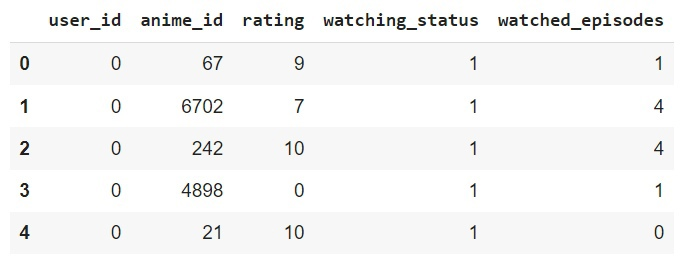
\includegraphics[width=0.8\linewidth]{disc1.png}
	
	\caption{Таблица animelist.csv}
	
	\label{fig:d1}
	
\end{figure}
 \subsubsection{Описание anime.csv.}
 В данном датасете 35 столбцов, большинство из них несут различную информацию про каждое аниме, поэтому опишем наиболее значительные данные для дальнейшей работы:
 \begin{itemize}
	\item \verb|MAL_ID| --- id аниме в списке (int),
	\item \verb|Name| --- полное английское название аниме (string),
	\item \verb|score| --- средняя оценка аниме от всех пользователей в базе данных MyAnimelist (float),
	\item \verb|genres| --- разделенный запятыми список жанров для этого аниме (string),
	\item \verb|type| --- фильм, сериал, дополнительная серия и тд. (string),
	\item \verb|episodes| --- количество частей (int),
	\item \verb|aired| --- дата трансляции (date),
	\item \verb|premiered| --- дата премьеры (date),
	\item \verb|rating| --- возрастной рейтинг (string),
	\item \verb|Popularity| --- позиция по количеству пользователей, которые добавили аниме в свой список (int),
	\item \verb|score-1 - score-10| --- количество зрителей, поставивших от 1 до 10 соответственно (float).
\end{itemize}

\verb|MAL_ID| в anime.csv и \verb|anime_id| в animelist.csv связаны, т.е. под \verb|anime_id| во второй таблице скрывается именно то аниме, которое будет найдено по 
тому же id в первой таблице.

\subsubsection{Описание anime$\_$with$\_$synopsis.csv.}

Данный датасет представляет собой краткий обзор для каждого аниме.

\begin{itemize}
	\item \verb|MAL_ID| --- id аниме в списке (int),
	\item \verb|Name| --- полное английское название аниме (string),
	\item \verb|score| --- средняя оценка аниме от всех пользователей в базе данных MyAnimelist (float),
	\item \verb|genres| --- разделенный запятыми список жанров для этого аниме (string),
	\item \verb|sypnopsis| --- описание аниме.
\end{itemize}

\verb|MAL_ID| аналогично связан с первой таблицей.

\subsection{Разведочный анализ}

Первоначально был изменен размер данных, чтобы учитывать более релевантных пользователей:

\begin{minted}[fontsize=\small, breaklines=true, linenos]{python}
n_ratings = rating_df['user_id'].value_counts()
rating_df = rating_df[rating_df['user_id'].isin(n_ratings[n_ratings >= 1000].index)]
\end{minted}

В результате работа будет производится с датасетом размером 11366011 строк.

Таблица распредения данных выглядит следующим образом:

\begin{figure}[h]

	\centering
	
	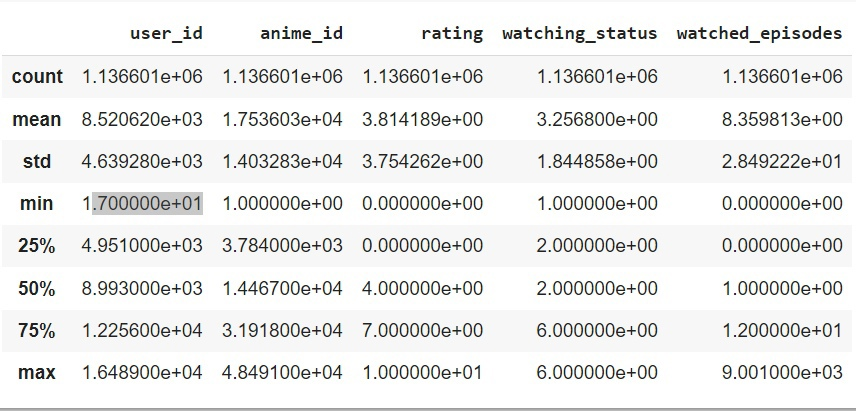
\includegraphics[width=0.8\linewidth]{analis1.png}
	
	\caption{Таблица распределения данных в rating\_df}
	
	\label{fig:a1}
	
\end{figure}

Столбец \verb|rating| вызывает наибольший интерес для данного исследования. Стандартное отклонение и среднее значение примерно равно,
 это можно трактовать как то, что данные в этом столбцы равномерно распределены вокруг среднего значения, 
 т. е. нет большого перевеса в одно из значений. Это подтверждают и значения квантиля этого столбца.

Пропуски и дубликаты в таблице отсутствуют.

\begin{figure}[H]

	\centering
	
	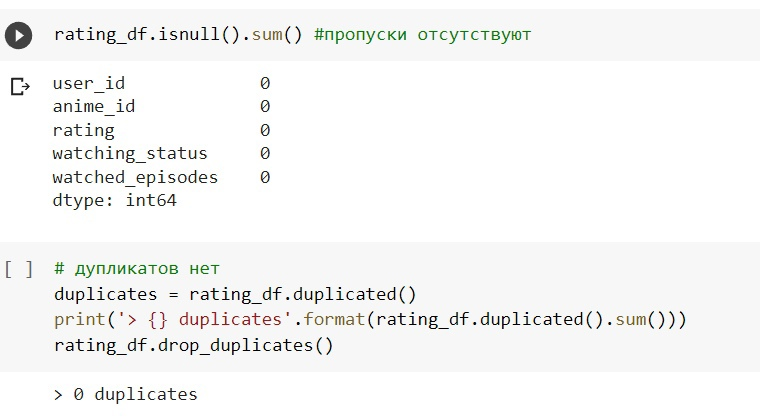
\includegraphics[width=0.8\linewidth]{analis2.png}
	
	\caption{Поиск пропусков и дубликатов}
	
	\label{fig:a2}
	
\end{figure}

Распределение столбца \verb|rating| было изучено на данном графике:
\begin{figure}[h]

	\centering
	
	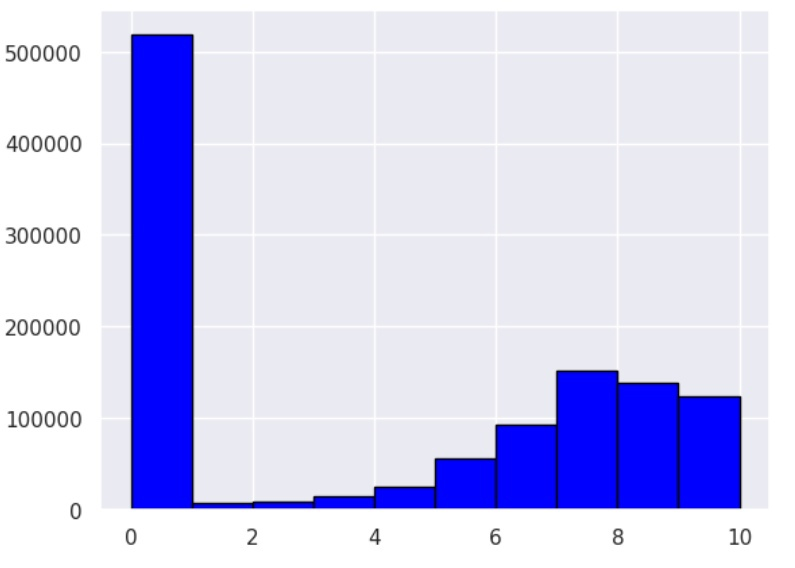
\includegraphics[width=0.8\linewidth]{analis3.png}
	
	\caption{Распределение rating}
	
	\label{fig:a3}
	
\end{figure}


Отметка \verb|rating| = 0 выставляется, если пользователь не поставил оценку, этот вариант преобладает над другими. Кроме того, можно заметить,
 что пользователя чаще ставят оценку ``выше среднего''. Можно предположить, что среднее значение более низкое, так как нулевой рейтинг портит эту статистику.

Был рассмотрен параметр \verb|watch_episodes|, для того чтобы проверить все ли аниме имеют корректное количество эпизодов:

\begin{figure}[ht]

	\centering
	
	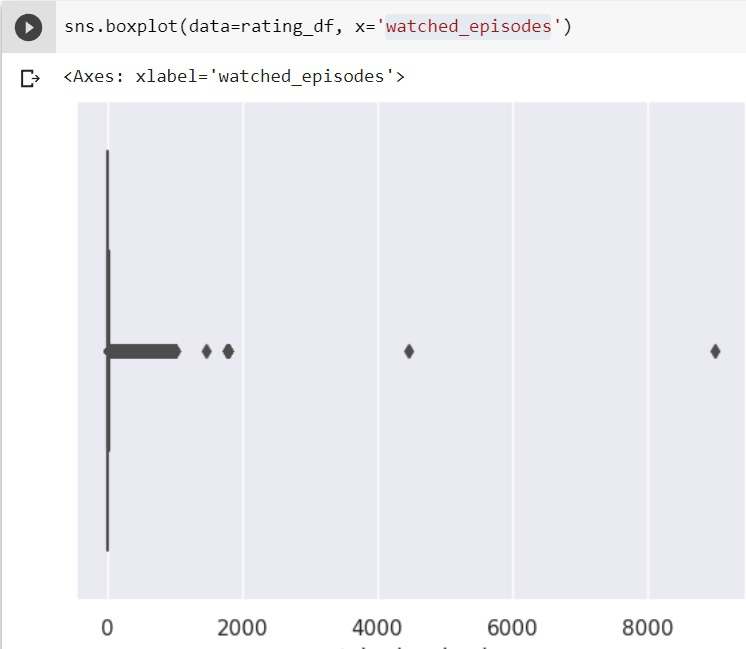
\includegraphics[width=0.8\linewidth]{analis4.png}
	
	\caption{boxplot столбца watch\_episodes}
	
	\label{fig:a4}
	
\end{figure}


Можно заметить несколько выбросов на графике. Данный вывод сделан из данных из-за того, что аниме с самым большим количеством серий насчитывает около 8500 эпизодов.

Было рассмотрено количество ненулевых оценок, которые ставят пользователи.
 Берется десять наибольших (слева --- id пользователя, справа --- количество ненулевых оценок):

 \begin{figure}[H]

	\centering
	
	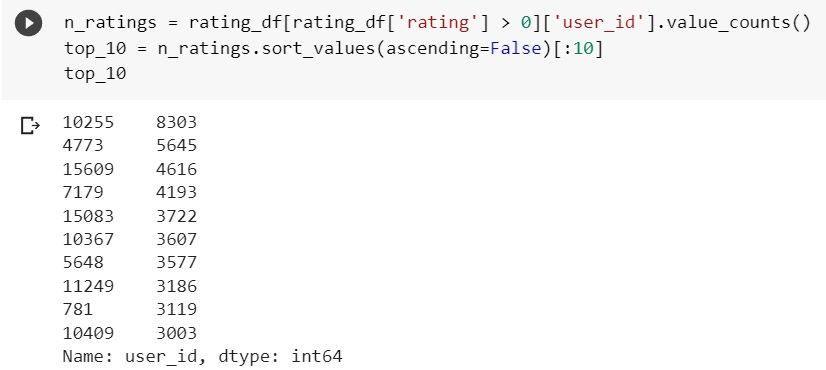
\includegraphics[width=0.8\linewidth]{analis5.png}
	
	\caption{Количество ненулевых оценок от пользователей}
	
	\label{fig:a5}
	
\end{figure}


Разрыв в значениях между первым и последним сильно отличаются, то есть некоторые
 пользователи будут иметь намного больше веса в системе, чем другие.

Были рассмотрены аналогичные сведения об аниме:

\begin{figure}[H]

	\centering
	
	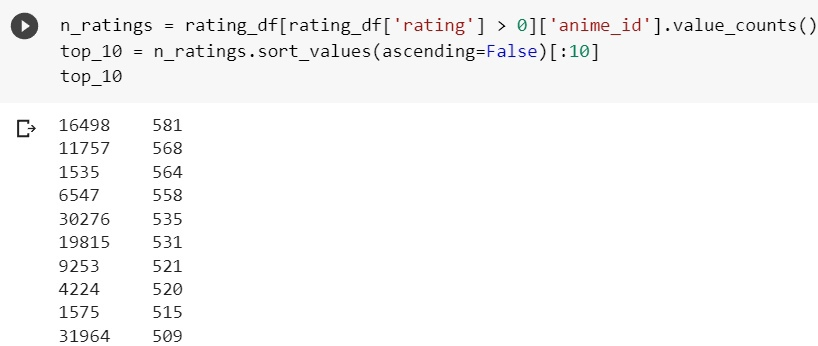
\includegraphics[width=0.8\linewidth]{analis6.png}
	
	\caption{Количество ненулевых оценок у аниме}
	
	\label{fig:a6}
	
\end{figure}

Количество ненулевых оценок распределено более равномерно, возможно, в системе некоторые аниме не будут чаще предлагаться,
 чем другие, только потому что их больше людей оценило.

Это может быть связано с тем, что количество аниме сильно больше, чем пользователей:

\begin{figure}[h]

	\centering
	
	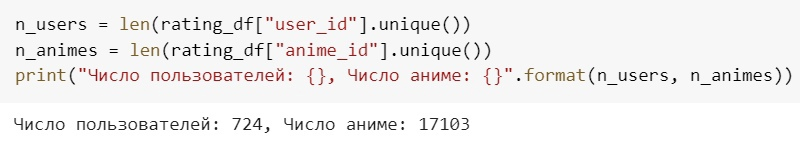
\includegraphics[width=0.8\linewidth]{analis7.png}
	
	\caption{Число уникальных пользователей и аниме}
	
	\label{fig:a7}
	
\end{figure}


\subsection{Предобработка данных}
Данные изначально не требуют больших изменений (отсутствуют пропуски, дубликаты, все значения --- int, \verb|rating| изменяется в определенном диапазоне). Однако в ходе разведочного анализа 
были обнаружены выбросы --- их необходимо удалить:

\begin{minted}[fontsize=\small, breaklines=true, linenos]{python}
rating_df = rating_df[rating_df['watched_episodes'] < 9000]
\end{minted}

Также существуют проблема, важная для рекомендательной системы. В таблице существуют пользователи, которые оценили абсолютно все аниме на 0, и аниме, которые все пользователи оценили на 0.  Такие данные не несут никакой полезной информации, и, более того, могут помешать дальнейшему обучению, поэтому их следует удалить:
\begin{minted}[fontsize=\small, breaklines=true, linenos]{python}
grouped = rating_df.groupby(['user_id']).agg({'rating': 'mean'})
grouped = grouped.loc[grouped['rating'] == 0]
user_ids = grouped['user_id'].unique()
rating_df = rating_df.loc[~rating_df['user_id'].isin(user_ids)]
grouped = rating_df.groupby(['anime_id']).agg({'rating': 'mean'})
grouped = grouped.loc[grouped['rating'] == 0]
user_ids = grouped['anime_id'].unique()
rating_df = rating_df.loc[~rating_df['anime_id'].isin(user_ids)]
\end{minted}

\subsection{Разработка и анализ моделей}
Как описано в разведочном анализе, целевая переменная --- рейтинг, который принимает целочисленные значения от 1 до 10. В данной работе проблема формулируется как пример обучения с учителем, где нужно предсказать рейтинг, учитывая пользователя и аниме. Хотя рейтинг принимает дискретные значение в диапазоне [0;10], имеет смысл сформулировать проблему, как задачу регрессии. Так следует поступить, поскольку в случае если модель классификации будет предсказывать оценку аниме с истинным рейтингом 10, то и оценка 9,
 и оценка 1 будут интерпретированы одинаково --- как неверный класс. В отличие от этого регрессионная модель наказывает за второй ответ больше чем за первый и это поведение подходит для данной задачи больше.

Первоначально для анализа необходимо выбрать метрику. В данной работе предлагается использовать \verb|RMSE| (среднеквадратичную ошибку) для сравнения качества предсказаний  моделей, как указано в источнике 
% [https://smltar.com/mlregression.html].

Как было сказано ранее, первая построенная модель --- базовая. Подсчитанные результаты будут использоваться как отправная точка для того, чтобы понять смогли ли мы улучшить результаты.

Разработанные в данном исследовании модели будет принимать id пользователя (\verb|user_id|) и id аниме (\verb|anime_id|), а возвращать число с плавающей точкой --- рейтинг.

Определим функцию для базовой модели:
\begin{minted}[fontsize=\small, breaklines=true, linenos]{python}
def base_model(user_id, anime_id):
  	return 5.0
\end{minted}

Также создадим функцию для подсчета средней квадратической ошибки на данных, где в качестве параметра выступает модель:


\begin{minted}[fontsize=\small, breaklines=true, linenos]{python}
from sklearn.metrics import mean_squared_error
def score(anime_model):
  id_pairs = zip(X_test['user_id'], X_test['anime_id'])
  y_pred = np.array([anime_model(user, anime) for (user, anime) in id_pairs])
  y_true = np.array(X_test['rating'])
  return mean_squared_error(y_true, y_pred, squared=False)
	\end{minted}

Здесь на строке 3 создаются пары из \verb|user_id| и \verb|model_id|, которые будем передавать на вход модели. Затем на строке 4 вычисляется
 предсказанный рейтинг путем последовательной передачи пар в модель. После этого на следующей строке извлекается целевой признак из тестовых данных,
  а затем на строке 6 производится подсчет \verb|RMSE| с помощью функции \verb|mean_squared_error| библиотеки \verb|sklearn|, которая была подключена на строке 1.

Запустив разработанную функцию для базовой модели, получаем показатель меры \verb|RMSE| равный 4,17.

\subsection{Модель на основе среднего значения}

Начинаем применять подход коллаборативной фильтрации основанной на пользователях. Для этого первоначально подготовим матрицу, где строка будет представлять id пользователя x, столбец id аниме y, а на пересечении стоять оценка, данная пользователем x аниме y. Для построения такой таблицы воспользуемся функцией
 \verb|pivot_table| библиотеки pandas.

\begin{minted}[fontsize=\small, breaklines=true, linenos]{python}
	r_matrix = X_train.pivot_table(values='rating', index = 'user_id', columns='anime_id')
\end{minted}



\begin{minted}[fontsize=\small, breaklines=true, linenos]{python}
r_matrix = X_train.pivot_table(values='rating', index = 'user_id', columns='anime_id')
\end{minted}

В этой реализации опробуем модель, которая будет выводить среднюю оценку между всеми пользователями, 
которые его оценят. Все пользователи будут считаться равными. Иными словами, рейтингу каждого пользователя присваивается равный вес.

Учтем случай, что некоторые аниме попали только в тестовый набор: в таком случае как и в базовой модели установим рейтинг 5.

\begin{minted}[fontsize=\small, breaklines=true, linenos]{python}
def mean_model(user_id, anime_id):
  if anime_id in r_matrix:
    mean_raiting = r_matrix[anime_id].mean()
  else:
    mean_raiting = 5.0
  return mean_raiting

\end{minted}

Метрика RSME для этой модели составляет 4.03.

Видим, что среднеквадратическое отклонение уменьшилось, следовательно качество предсказаний улучшилось.


\subsection{Модель на основе cредневзвешенной оценки}
В данной модели будем отдавать больше предпочтения тем пользователям, чьи оценки похожи на рассматриваемого пользователя больше.

Поэтому дополним предыдущую модель весовым коэффициентом:

$$\bar r_{ua} = \frac{1}{\sum_{u', u' \neq u} s_{uu'}}  \sum_{u', u' \neq u} s_{uu'}r_{u'a}$$, где 

В теоретической части было представлено обоснование использование косинусной метрики в качестве $s$. Для работы с косинусной метрикой подключим функцию \verb|cosine_similarity| библиотеки \verb|sklearn|.

\begin{minted}[fontsize=\small, breaklines=true, linenos]{python}
from sklearn.metrics.pairwise import cosine_similarity
\end{minted}

Функция \verb|cosine_sim| не работает со значениями \verb|NaN| которые есть в нашей матрице. Заменим их на 0:

\begin{minted}[fontsize=\small, breaklines=true, linenos]{python}
r_matrix_notnull = r_matrix.copy().fillna(0)
\end{minted}

C помощью функции построим новую матрицу косинусного сходства между пользователями:

\begin{minted}[fontsize=\small, breaklines=true, linenos]{python}
cosine_sim = pd.DataFrame(cosine_sim, index=r_matrix.index, columns=r_matrix.index)
\end{minted}

Теперь по аналогии с предыдущей моделью рассчитаем средневзвешенные оценки. Однако теперь еще необходимо учитывать только ненулевые оценки косинусного сходства. 
То есть нам нужно избегать пользователей, не оценивших аниме.

\begin{minted}[fontsize=\small, breaklines=true, linenos]{python}
def model_weightmean(user_id, anime_id):
  if anime_id in r_matrix:
    similars = cosine_sim[user_id]
    # оценки пользователей для аниме
    m_ratings = r_matrix[anime_id]
    # запишем индексы тех элементов, что имеют нулевое косинусное сходство
    idx = m_ratings[m_ratings.isnull()].index
    #удалим оценки, которые содержат Nan
    m_ratings = m_ratings.dropna()
    # удалим косинусное сходство элементов, которые содержат Nan
    similars = similars.drop(idx)
    # рассчитаем средневзвешенное по формуле
    weightmean = np.dot(similars, m_ratings)/ similars.sum()
  else:
    weightmean = 5.0
  return weightmean
\end{minted}

Время обработки данной модели значительно больше, чем у предыдущей модели. Тем не менее удалось добиться (небольшого) улучшения показателя RSME равного 4.019.

\subsubsection{Модель кластеризации}

Попробуем построить модель на основе кластеризации.

Для кластеризации используем алгоритм k-средних, а затем будем использовать для рекомендаций только пользователей из одного кластера.

Нам необходимо решить следующие задачи:
\begin{itemize}
	\item Найти k-ближайших соседей, у которых есть рейтинг аниме a.
	\item Вывести средний рейтинг k пользователей для аниме a.
\end{itemize}

А также подберем гиперпараметры KNN, которыми выступают:
\begin{itemize}
	\item Число соседей (n$\_$neighbors),
	\item Метрика сходства --- Минковского или косинусная,
	\item Степень для метрики Минковского (p) --- 1 или 2 часто лучшие. Когда p = 1, это эквивалентно использованию \verb|manhattan_distance| (l1) и \verb|euclidean_distance| (l2) для p = 2.
\end{itemize}

\begin{minted}[fontsize=\small, breaklines=true, linenos]{python}
def model_weightmean(user_id, anime_id):
from sklearn.neighbors import KNeighborsRegressor
from sklearn.model_selection import GridSearchCV


knn = KNeighborsRegressor()


param_grid = [
{'n_neighbors': range(1, 10, 1), 'metric' : ['cosine']},
{'n_neighbors': range(1, 10, 1), 'metric' : ['minkowski'],
'p': [1, 2, 3]},
]
grid_search = GridSearchCV(knn, param_grid, cv=5, n_jobs = -1, verbose = 1)
best_model = grid_search.fit(X_train, y_train)

\end{minted}

В данном коде импортируется регрессионный алгоритм KNN и оценщик \verb|GridSearchCV| для подбора параметров из библиотеки \verb|sklearn| (строки 1-2). В строке 4 создается регрессор. На 6-10 строке приведен словарь гиперпараметров на которых будет работать оценщик. Опробуем регрессор
 с косинусной метрикой и числом соседей от 1 до 10 с шагом 1, а также регрессор с метрикой Минковского, степенью этой метрики от 1 до 3, а также с числом
  соседей от 1 до 10 с шагом 1. Далее объявляется оценщик с заданным словарем гиперпараметров и параметром $cv = 5$. Это означает, что здесь используется пятикратная кросс-валидация. Следовательно датасет делится на пять частей, где 4 используются для обучения, 
  а пятый для проверки. Таким образом оценщик проходит датасет пять раз, чтобы каждая часть была проверочной ровно один раз.

После обучения наилучшими параметрами оценщик выбрал: косинусную метрику, степень метрики 2, число соседей равное одному:

\begin{minted}[fontsize=\small, breaklines=true, linenos]{python}
print('Best metric:', best_model.best_estimator_.get_params()['metric'])
print('Best p:', best_model.best_estimator_.get_params()['p'])
print('Best n_neighbors:', best_model.best_estimator_.get_params()['n_neighbors'])
\end{minted}

Сделаем предсказание на тестовой выборке и оценим мерой \verb|RMSE|:

\begin{minted}[fontsize=\small, breaklines=true, linenos]{python}
y_true = np.array(X_test['rating'])
np.array(X_test['rating'])
y_pred = best_model.predict(X_test)
mean_squared_error(y_true, y_pred, squared=False)
\end{minted}

Наблюдаем, что RSME, полученный этой моделью, равен 0.94. Это лучший результат, который был достигнут.
Полный код рекомендательной системы методом KNN представлен в приложении \ref{pr1}.
\subsubsection{Нейронная сеть}

Построение модели нейронной сети, как и описывалось в теории, начинается с уровня \verb|embedding|. Здесь векторы пользователей и аниме уплотняются и преобразуются: 

\begin{minted}[fontsize=\small, breaklines=true, linenos]{python}
embedding_size = 128
 user = Input(name = 'user', shape = [1])
 user_embedding = Embedding(name = 'user_embedding',
                       input_dim = n_users, 
                       output_dim = embedding_size)(user)
 anime = Input(name = 'anime', shape = [1])
 anime_embedding = Embedding(name = 'anime_embedding',
                       input_dim = n_animes, 
                       output_dim = embedding_size)(anime)

\end{minted}

Далее они объединяются и выравниваются: 

\begin{minted}[fontsize=\small, breaklines=true, linenos]{python}
x = Dot(name = 'dot_product', normalize = True, axes = 2)([user_embedding, anime_embedding])
x = Flatten()(x)
\end{minted}

\begin{minted}[fontsize=\small, breaklines=true, linenos]{python}
x = Dense(1, kernel_initializer='he_normal')(x)
x = BatchNormalization()(x)
\end{minted}

Наконец, последним слоем является функция активации.  Другие функции не рассматриваются (например, elu, relu), так как такая вариация занимает слишком много времени для обучения (порядка 6 часов), а все рассмотренные функции, кроме сигмоиды, вызывают переобучение. Поэтому было решено использовать только один вариант.

\begin{minted}[fontsize=\small, breaklines=true, linenos]{python}
x = Activation(hp.Choice('activation', values=['sigmoid']))(x)  
\end{minted}

В качестве функции потерь была выбрана бинарная кросс-энтропия. Бинарная кросс-энтропия показывает, насколько отличается
 изначальный рейтинг от рейтинга, предсказанного нейросетью. 

В качестве оптимизатора предложено три варианта. Таким образом 
будет построено три модели нейронной сети:
\begin{minted}[fontsize=\small, breaklines=true, linenos]{python}
model.compile(loss='binary_crossentropy', metrics=["mae", "mse"], optimizer=hp.Choice('optimizer', values=['adam','rmsprop','SGD']))  
\end{minted}

Для обучения использован \verb|BayesianOptimization|, в качестве метрики для оптимизации выбрана mse, т.к. именно она позже будет использована для сравнения с результатами другого способа построения рекомендательной системы.
\begin{minted}[fontsize=\small, breaklines=true, linenos]{python}
tuner = BayesianOptimization(
    RecommenderNet,                 
    objective='val_mse',                              
    max_trials=10,              
    directory='test_directory'   
    )
\end{minted}

Обучение производится с использование следующих параметров:

\begin{minted}[fontsize=\small, breaklines=true, linenos]{python}
tuner.search(X_train_array,                  
             y_train,                  
             batch_size=10000,          
             epochs=10,                 
             validation_split=0.2,   
             )

\end{minted}

Изначально сеть обучалась на 20 эпохах, но первые попытки показали, что после 10-ой эпохи во всех моделях улучшение метрик прекращается, поэтому было решено уменьшить это значение.

Результаты обучения следующие: 

\begin{figure}[ht!]

	\centering
	
	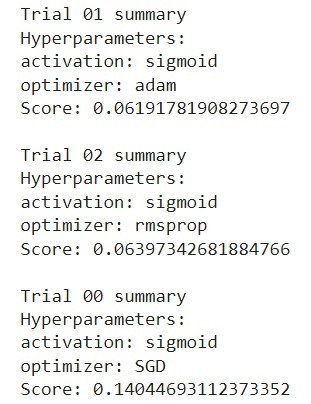
\includegraphics[width=0.3\linewidth]{pract1.png}
	
	\caption{Результаты обучения нейронной сети}
	
	\label{fig:p1}
	
\end{figure}

Лучше всего себя показала модель с оптимизатором Adam, хотя и результаты с rmsprop не сильно хуже. Score вышел действительно маленьким (меньше 0.1) это говорит о правильно составленной нейронной сети и удачном подборе параметров. Осталось проверить эти результаты на тестовой выборке:


\begin{figure}[ht!]

	\centering
	
	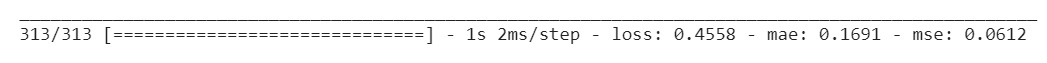
\includegraphics[width=0.8\linewidth]{pract2.png}
	
	\caption{Тестирование Adam}
	
	\label{fig:p2}
	
\end{figure}

\begin{figure}[ht!]

	\centering
	
	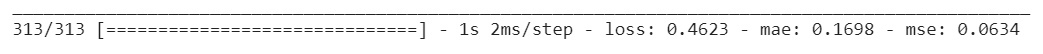
\includegraphics[width=0.8\linewidth]{pract3.png}
	
	\caption{Тестирование rmsprop}
	
	\label{fig:p3}
	
\end{figure}

\begin{figure}[ht!]

	\centering
	
	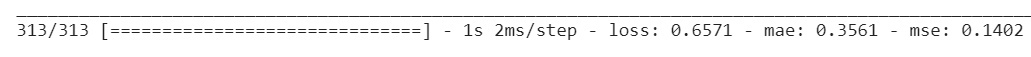
\includegraphics[width=0.8\linewidth]{pract4.png}
	
	\caption{Тестирование SGD}
	
	\label{fig:p4}
	
\end{figure}

Проверка на тестовых данных подтвердила результаты обучения.
Полный код рекомендательной системы на нейросети представлен в приложении \ref{pr2}.

\subsection{Результаты}
В результате проделанной работы были изучены и реализованы различные методы построения рекомендательной системы. 

Сравнение методов построения системы производится с помощью меры RMSE. В нейронной сети подсчитывался параметр MSE, однако из него легко получить требуемый для сравнения:
$$RMSE = \sqrt{MSE}$$
Таблица сравнения построенных методов в работе:

\begin{table}[!ht]
	\small
	\caption{Результат сокращения словарей неисправностей при помощи масок} \label{table-1}
	\begin{tabular}{|l|c|}
		\hline Название метода & Мера RMSE\\
		\hline Базовый & 4.176227963 \\
		\hline Коллаборативный на основе среднего значения & 4.019703832 \\
		\hline Коллаборативный на основе средневзвешенного значения & 4.019703832 \\
		\hline Нейронная сеть (Adam) & 0.247386338 \\
		\hline Нейронная сеть (rmsprop) & 0.252922913 \\
		\hline Нейронная сеть (SGD) & 0.374432905 \\
		
		\hline
	\end{tabular}
\end{table}

\subsection{Практическая деятельность}
Внедрение результата в практическую деятельность в рекомендательной системе можно представить наглядно. Для этого строится функция предсказания. Построенные модели позволяют показать два варианта систем: Item-based и user-based.

\subsubsection{Item-based на основе нейронной сети}
Для начала получаются веса аниме из модели:

\begin{minted}[fontsize=\small, breaklines=true, linenos]{python}
def extract_weights(name, model):
    weight_layer = model.get_layer(name)
    weights = weight_layer.get_weights()[0]
    weights = weights / np.linalg.norm(weights, axis = 1).reshape((-1, 1))
    return weights


anime_weights = extract_weights('anime_embedding', model)
\end{minted}

Именно на основе этих значений будет строится вектор расстояний до различных аниме, которые отражают схожесть.

В функции вектор со всеми весами умножается на вес текущего аниме для нахождения вектора расстояний. Далее берется n самых больших и наиболее подходящих для заявленного аниме:

\begin{minted}[fontsize=\small, breaklines=true, linenos]{python}
index = getAnimeFrame(name).anime_id.values[0]
weights = anime_weights
dists = np.dot(weights, weights[index])
sorted_dists = np.argsort(dists)          
if neg:
  closest = sorted_dists[:(n + 1)]
else:
  closest = sorted_dists[(-n - 1):]
\end{minted}

Результатом вызова функции

\begin{minted}[fontsize=\small, breaklines=true, linenos]{python}
 find_similar_animes('xxxHOLiC', n=10,  neg=False)
\end{minted}

будет следующая таблица:
\begin{figure}[H]

	\centering
	
	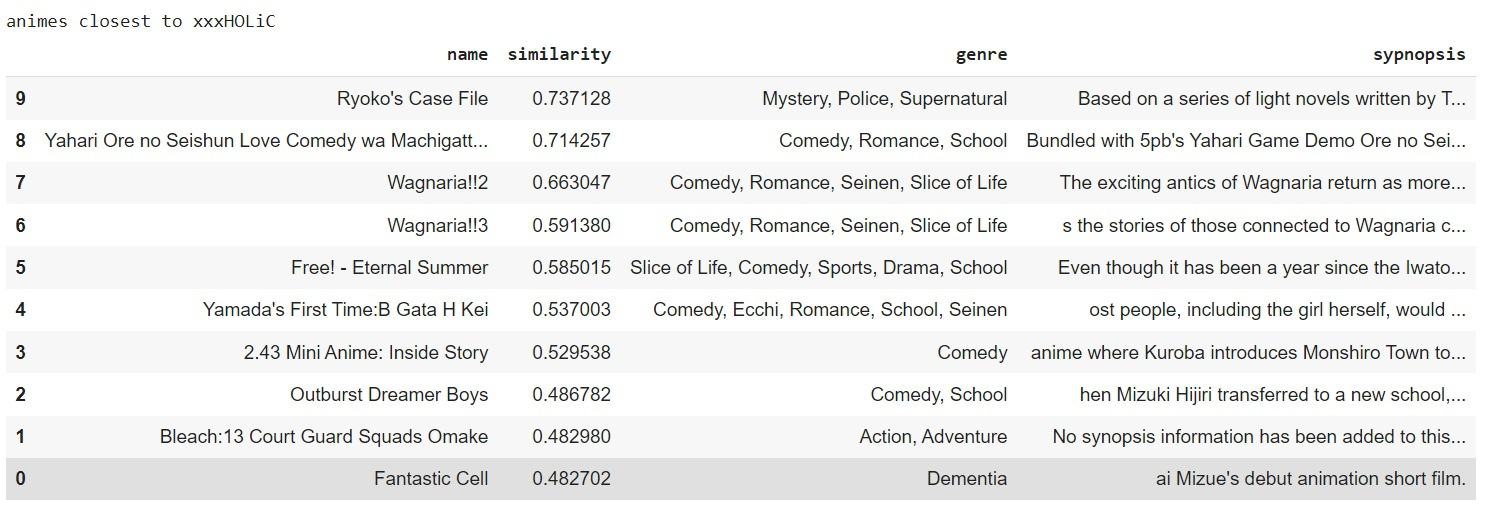
\includegraphics[width=0.8\linewidth]{res1.png}
	
	\caption{Рекомендации от нейронной сети}
	
	\label{fig:r1}
	
\end{figure}

Весь код можно посмотреть в приложении \ref{pr3}.


\subsubsection{User-based подход в коллаборативном KNN}
Для использования модели создан метод predict. На вход он получает id пользователя и по нему рекомендует аниме. 

\begin{minted}[fontsize=\small, breaklines=true, linenos]{python}
knn = KNeighborsRegressor(metric='cosine', p = 2, n_neighbors=1)
n_knn = knn.fit(X_train, y_train)
def predict(user_id):
  test_set = X[X['user_id'] == user_id]
  distances, indeces =  n_knn.kneighbors(test_set)
  final_table = pd.DataFrame(distances, columns = ['distance'])
  final_table['index'] = indeces
  final_table = final_table.set_index('index')
  result = final_table.join(X_train,on='index')
  result = result.join(synopsis_df, on='anime_id')
  return result[['distance','Name', 'Score', 'Genres']].head(5)
\end{minted}

На строках 1-2 производится создание обучение модели с подобранными гиперпараметрами. В строке 4 выбираются те аниме из датасета, что были оценены выбранным пользователем. Функция kneighbors возвращает из обученного KNN расстояния и индексы (в обучающем наборе) сходных записей. На строках 6-8 создается первоначальная таблица, куда записываются полученные из алгоритма расстояния и индексы.
 Затем на строках 9-10 по индексу данная таблица объединяется с другой, 
 содержащей подробную информацию о рекомендуемом аниме.
  В итоге метод возвращает таблицу, где представлен индекс аниме,
   его метрика, название, оценка и метки жанров. К примеру функция для пользователя с id 573 вернет:

   \begin{figure}[h]

	\centering
	
	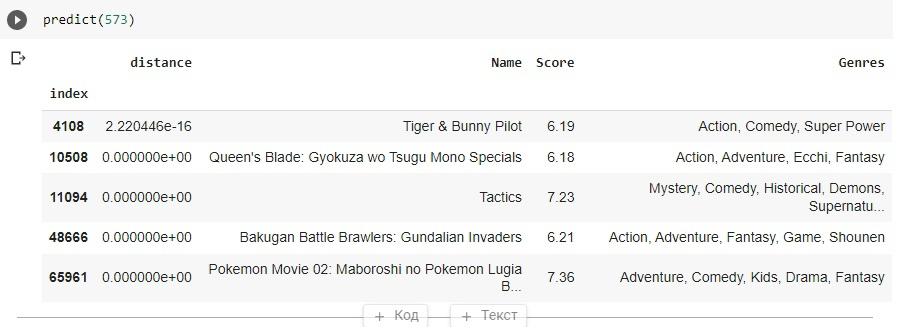
\includegraphics[width=0.8\linewidth]{res2.png}
	
	\caption{Рекомендации KNN}
	
	\label{fig:r2}
	
\end{figure}



% Раздел "Заключение"
\conclusion
В данной работе были рассмотрены различные методы построения коллаборативной рекомендательной системы.
 Для улучшения качества рекомендаций были использованы модели на основе среднего значения,
  средневзвешенной оценки, кластеризации и нейронной сети.

Было показано на практике построение таких моделей и выведена метрика их оценивания для
 сравнения их точности и возможностей. Кроме того реализованы функции, одна из которых
  выводит конкретному пользователю список рекомендуемых аниме. Она основана 
  на методе кластеризации коллаборационной системы. Другая функция принимает название аниме
   и выводит список объектов, похожих на него. Ее работа основана на нейронной сети.

В процессе исследования было выявлено, что эти методы имеют свои плюсы и минусы.
 Например, модель на основе среднего значения может быть не очень точной, поскольку
  она не учитывает предпочтения пользователей. С другой стороны, нейронная сеть показала очень
   хорошие результаты, но ее требования к производительности могут быть весьма высокими.

Тем не менее, на основании проведенных исследований можно заключить, что каждый из рассмотренных
 методов может быть полезным в зависимости от конкретных задач и условий. К примеру,
  метод кластеризации может использоваться для повышения точности рекомендаций в случае,
   если у нас нет достаточного количества данных для применения более сложного алгоритма.

В целом, эта работа показала, что построение коллаборативной рекомендательной системы 
является сложной задачей, требующей постоянного исследования и улучшения. Однако, 
применение вышеуказанных методов имеют большой потенциал для оптимизации рекомендаций и создания 
более удобного пользовательского опыта.

Работа над проектом была распределена следующим образом: 
исследование данных, разведочный анализ и предобработка производились совместно,
 так как это имеет большое значение для методов обучения. Существуют принципиальные действия,
  которые необходимо выполнить для обоих практических частей проекта, это можно было отследить
   лишь посредством коллективной разработки.

Изучение методов, связанных с различными оценками и кластеризацией данных,
 и, соответственно, их реализация, были выполнены Озеровым Данилой.
  А построение модели нейронной сети, ее реализация и обучение произвела Медведева Татьяна.
   Соответственно была написана и теоретическая часть.


%Библиографический список, составленный вручную, без использования BibTeX
%
%\begin{thebibliography}{99}
%  \bibitem{Ione} Источник 1.
%  \bibitem{Itwo} Источник 2
%\end{thebibliography}

%Библиографический список, составленный с помощью BibTeX
%
\bibliographystyle{gost780uv}
\bibliography{thesis}

% Окончание основного документа и начало приложений
% Каждая последующая секция документа будет являться приложением
\appendix

\section{Модель на основе среднего значения, средневзвешенной оценки, кластеризации}

\label{pr1}
\begin{minted}[fontsize=\small, breaklines=true, linenos]{python}
#В этой реализации опробуем модель, которая будет выводить 
#среднюю оценку между всеми пользователями, которые его оценят. Все пользователи будут считаться равными.
# Иными словами, рейтингу каждого пользователя присваивается равный вес.

#Учтем случай, что некоторые аниме попали только в тестовый набор: в таком случае как и в "глупой" модели установим рейтинг 5.
def mean_model(user_id, anime_id):
  if anime_id in r_matrix:
    mean_raiting = r_matrix[anime_id].mean()
  else:
    mean_raiting = 5.0
  return mean_raiting

score(mean_model)

#Средневзвешенная
# В данной модели будем отдавать больше предпочтения тем пользователям,
# чьи оценки похожи на рассматриваемого пользователя больше.
from sklearn.metrics.pairwise import cosine_similarity

#Функция cosine_similarity не работает со значениями Nan. Поэтому заменим их на 0.
r_matrix_notnull = r_matrix.copy().fillna(0)
cosine_sim = cosine_similarity(r_matrix_notnull, r_matrix_notnull)

cosine_sim = pd.DataFrame(cosine_sim, index=r_matrix.index, columns=r_matrix.index)

def model_weightmean(user_id, anime_id):

  if anime_id in r_matrix:
    similars = cosine_sim[user_id]
    # оценки пользователей для аниме
    m_ratings = r_matrix[anime_id]
    # запишем индексы тех элементов, что имеют нулевое косинусное сходство
    idx = m_ratings[m_ratings.isnull()].index
    #удалим оценки, которые содержат Nan
    m_ratings = m_ratings.dropna()
    # удалим косинусное сходство элементов, которые содержат Nan
    similars = similars.drop(idx)
    # расчитаем средневзвешенное по формуле
    weightmean = np.dot(similars, m_ratings)/ similars.sum()
  else:
    weightmean = 5.0
  return weightmean

score(model_weightmean)

# Кластеризация
from sklearn.neighbors import KNeighborsRegressor
from sklearn.model_selection import GridSearchCV

knn = KNeighborsRegressor()

param_grid = [
{'n_neighbors': range(1, 10, 1), 'metric' : ['cosine']},
{'n_neighbors': range(1, 10, 1), 'metric' : ['minkowski'],
'p': [1, 2, 3]},
]
grid_search = GridSearchCV(knn, param_grid, cv=5, n_jobs = -1, verbose = 1)
best_model = grid_search.fit(X_train, y_train)

y_true = np.array(X_test['rating'])
np.array(X_test['rating'])
y_pred = best_model.predict(X_test)

#обучим с подобранными параметрами
knn = KNeighborsRegressor(metric='cosine', p = 2, n_neighbors=1)

n_knn = knn.fit(X_train, y_train)
def predict(user_id):
  # находим оцененные аниме нашего пользоватлея
  test_set = X[X['user_id'] == user_id]
  # выводим из обученного Knn расстояния и индексы схожих аниме
  distances, indeces =  n_knn.kneighbors(test_set)
  # создаем таблицу с растояниями и индексами
  final_table = pd.DataFrame(distances, columns = ['distance'])
  final_table['index'] = indeces
  final_table = final_table.set_index('index')
  # добавляем в таблицу название, оценку и жанр
  result = final_table.join(X_train,on='index')
  result = result.join(synopsis_df, on='anime_id')
  # выводим 5 значений
  return result[['distance','Name', 'Score', 'Genres']].head(5)
\end{minted}

\section{Рекомендательная система на нейросети}
\label{pr2}
\begin{minted}[fontsize=\small, breaklines=true, linenos]{python}
import tensorflow as tf
from tensorflow.keras import layers
from tensorflow.keras.models import Model
from tensorflow.keras.optimizers import Adam
from tensorflow.keras.layers import Add, Activation, Lambda, BatchNormalization, Concatenate, Dropout, Input, Embedding, Dot, Reshape, Dense, Flatten
from tensorflow.keras.datasets import fashion_mnist
from tensorflow.keras.models import Sequential
from tensorflow.keras.layers import Dense
from tensorflow.keras import utils
from keras_tuner.tuners import BayesianOptimization
import numpy as np

def RecommenderNet(hp):
    embedding_size = 128
    user = Input(name = 'user', shape = [1])
    # Превращает положительные целые числа (индексы) в плотные векторы фиксированного размера.
    # совершаем эту операцию с обоими стобцами
    user_embedding = Embedding(name = 'user_embedding',
                       input_dim = n_users, 
                       output_dim = embedding_size)(user)
    
    anime = Input(name = 'anime', shape = [1])
    anime_embedding = Embedding(name = 'anime_embedding',
                       input_dim = n_animes, 
                       output_dim = embedding_size)(anime)
    # вычисляем скалярное произведение между двумя получившимися векторами
    x = Dot(name = 'dot_product', normalize = True, axes = 2)([user_embedding, anime_embedding])
    # выравниваем массив выборки, превращая его из вида (x, y) (x * y = размер батча) в (x * y)
    x = Flatten()(x)
    # используем стандартный инициализатор 
    x = Dense(1, kernel_initializer='he_normal')(x)
    # нормализируем батчи
    x = BatchNormalization()(x)
    # в качестве функции активации используем сигмоиду
    # мы могли бы использовать другие функции активации
    # но при первом запуске всех допустимых функций (relu, elu и тд)
    # сигмоида сильно лучше работала, а время обучение составляло слишком большое число (порядка 6-ти часов)
    # поэтому было принято решения использовать только сигмоиду
    x = Activation(hp.Choice('activation', values=['sigmoid']))(x)
    
    model = Model(inputs=[user, anime], outputs=x)
    # компилируем, в качестве метрики используем mae и mse, в качестве оптимизатора - подбираем один из трех
    model.compile(loss='binary_crossentropy', metrics=["mae", "mse"], optimizer=hp.Choice('optimizer', values=['adam','rmsprop','SGD']))
    
    return model

	tuner = BayesianOptimization(
    RecommenderNet,                 # функция создания модели
    objective='val_mse',    # метрика, которую нужно оптимизировать -                             
    max_trials=10,               # максимальное количество запусков обучения 
    directory='test_directory'   # каталог, куда сохраняются обученные сети  
    )

	tuner.search_space_summary()

		# обучение модели
	batch_size = 10000 # тк размер выборки большой, выбираем батчи размером 10к
	tuner.search(X_train_array,                  # Данные для обучения
				y_train,                  # Правильные ответы
				batch_size=10000,           # Размер мини-выборки
				epochs=10,                # Количество эпох обучения 
				validation_split=0.2,    # Часть данных, которая будет использоваться для проверки
				)

	
	models = tuner.get_best_models(num_models=3)

	for model in models:
		model.summary()
		model.evaluate(X_test_array, y_test)
		print() 

\end{minted}

\section{Функция предсказания от нейросети}
\label{pr3}
\begin{minted}[fontsize=\small, breaklines=true, linenos]{python}
	#из модели извлекаем веса для аниме и пользователей и сохраняем в переменные
def extract_weights(name, model):
    weight_layer = model.get_layer(name)
    weights = weight_layer.get_weights()[0]
    weights = weights / np.linalg.norm(weights, axis = 1).reshape((-1, 1))
    return weights

anime_weights = extract_weights('anime_embedding', model)

# исправляем названия аниме
def getAnimeName(anime_id):
    #если нет названия аниме на английском, то ставим японское название
    name = df_anime[df.anime_id == anime_id].eng_version.values[0]
    if name == "Unknown":
        name = df_anime[df.anime_id == anime_id].Name.values[0] 
    return name
#переименовываем столбцы
df_anime.rename(columns= {'MAL_ID':'anime_id','English name':'eng_version'}, inplace = True)
#применяем функцию для исправления названия аниме
df_anime['eng_version'] = df_anime.anime_id.apply(lambda x: getAnimeName(x))
#сортируем аниме по средней оценке аниме от всех пользователей в базе данных 
df_anime.sort_values(by=['Score'], 
               inplace=True,
               ascending=False, 
               kind='quicksort',
               na_position='last')
#оставляем нужные столбцы
df_anime = df_anime[["anime_id", "eng_version", 
         "Score", "Genres", "Episodes", 
         "Type", "Premiered", "Members"]]

#функция для получения строки с аниме по названию или id
def getAnimeFrame(anime):
    if isinstance(anime, int):
        return df[df.anime_id == anime]
    if isinstance(anime, str):
        return df[df.eng_version == anime]

cols = ["MAL_ID", "Name", "Genres", "sypnopsis"]

#функция для получения строки с описанием аниме по названию или id
def getSypnopsis(anime):
    if isinstance(anime, int):
        return synopsis_df[synopsis_df.MAL_ID == anime].sypnopsis.values[0]
    if isinstance(anime, str):
        return synopsis_df[synopsis_df.Name == anime].sypnopsis.values[0]

#функция для вывода рекомендации аниме
def find_similar_animes(name, #название аниме или id
                        n=10, #количество аниме которые рекомендуем (по умолчанию 10)
                        return_dist=False, #выводим ли растояние (по умолчанию нет)
                        neg=False): #в каком порядке выводим список
    try:
        #записываем в переменные id аниме и вес
        index = getAnimeFrame(name).anime_id.values[0]
        weights = anime_weights
        #умножаем вектор со всеми весами на вес текущего аниме для нахождения вектора расстояний
        dists = np.dot(weights, weights[index])
        #сортируем его
        sorted_dists = np.argsort(dists)          
        #выбираем порядок вывода
        if neg:
            closest = sorted_dists[:(n + 1)]
        else:
            closest = sorted_dists[(-n - 1):]

        print('animes closest to {}'.format(name))
        #выводим вектор расстояний если нужно
        if return_dist:
            return dists, closest
        
        rindex = df

        SimilarityArr = []

        for close in closest:
            #для каждого аниме из списка берем описание, название, жанры и расстояние
            sypnopsis = getSypnopsis(index)
            anime_frame = getAnimeFrame(index)
            
            anime_name = anime_frame.eng_version.values[0]
            genre = anime_frame.Genres.values[0]
            similarity = dists[close]
            #после записываем в список параметры
            SimilarityArr.append({"anime_id": decoded_id, "name": anime_name,
                                  "similarity": similarity,"genre": genre,
                                  'sypnopsis': sypnopsis})
        #сортируем его по расстоянию и возвращаем из функции
        Frame = pd.DataFrame(SimilarityArr).sort_values(by="similarity", ascending=False)
        return Frame[Frame.anime_id != index].drop(['anime_id'], axis=1)

    except:
        print('{}!, Не найден в Аниме листе'.format(name))
\end{minted}


\end{document}
